% Standalone Overleaf-ready paper draft for BC_Tactile_Lab.
% Create a blank Overleaf project, replace main.tex with this entire file, and
% compile with pdfLaTeX. All \TBD{} entries require measured evidence.

\documentclass[10pt,twocolumn]{article}

\usepackage[margin=0.72in]{geometry}
\usepackage{amsmath,amssymb}
\usepackage{booktabs}
\usepackage{graphicx}
\usepackage[table]{xcolor}
\usepackage{microtype}
\usepackage[hidelinks]{hyperref}

\title{MosaicTouch: Heterogeneous Full-Hand Tactile Simulation\\
for Sim-to-Real Dexterous Manipulation}
\author{Anonymous Authors}
\date{}

\newcommand{\TBD}[1]{\textcolor{red}{[TBD: #1]}}

\begin{document}
\maketitle

\begin{abstract}
We present MosaicTouch, an integrated full-hand tactile simulation framework
that combines pressure sensing and visuo-tactile sensing for dexterous robotic
hands. Distributed pressure arrays cover the palm and finger links, while
curved visuo-tactile sensors at all five fingertips capture detailed local
contact. This complementary layout provides full-hand contact coverage without
sacrificing the geometric and tangential information available at the
fingertips. MosaicTouch represents touch using three signals that can be
recovered from the corresponding physical sensors: pressure maps for broad
contact coverage, penetration-depth maps for local contact geometry, and
marker-displacement fields for tangential interaction. For curved fingertips,
we construct the undeformed sensing surface from the hand geometry, track
contact history in three dimensions, and project dilation and shear through
spatially varying local tangent frames rather than assuming a planar sensor.
All pressure and visuo-tactile signals are computed in batches on the GPU and
exposed directly as policy observations, without photorealistic tactile
rendering during learning. We evaluate the framework through paired
real--simulation measurements of both sensor modalities, parallel simulation
benchmarks, tactile-observation ablations in reinforcement learning and
teacher--student behavior cloning, and direct policy transfer to the physical
hand. \TBD{Report pressure, depth, marker-motion, throughput, and real-robot
results after completing the experiments.}
\end{abstract}

\section{Introduction}
\label{sec:introduction}

Dexterous manipulation depends on contacts that are only partially observable
from external cameras.  This limitation is particularly severe during grasp
closure and in-hand manipulation, where the object is occluded by the hand and
contact may migrate from the fingertips to the intermediate phalanges or palm.
Large-area tactile skins provide broad contact coverage, but commonly expose
low-dimensional pressure measurements.  Vision-based tactile sensors provide
dense contact geometry and marker motion, but are usually installed only at the
fingertips because of their cameras, optics, and packaging.  Consequently, a
robotic hand often has to choose between broad coverage and rich local contact
information.

We present \emph{\TBD{system name}}, a heterogeneous full-hand tactile
simulation and real-robot framework that combines distributed pressure sensing
with curved fingertip visuo-tactile sensing.  The simulated hand mirrors the
physical sensor layout: pressure arrays cover the palm and non-distal finger
links, while five curved visuo-tactile fingertips provide local penetration
depth and marker displacement.  Rather than converting all sensors into a
photorealistic image, we retain representations that are close to the physical
measurement of each modality.  Pressure is represented as calibrated force
maps; fingertip contact geometry is represented as a penetration-depth map; and
tangential interaction is represented by a history-dependent marker
displacement field.  These signals share a batched GPU implementation and are
assembled into a common policy observation.

The central technical challenge is that existing fast marker-motion models are
usually formulated in a planar image frame, whereas our fingertip sensing
surface is curved.  We therefore construct a local tangent frame from the
sampled fingertip surface, track object-surface motion in three dimensions, and
project the resulting dilation and shear displacement into the sensor's
nonuniform image coordinates.  This preserves the efficient, history-dependent
contact model needed for parallel policy learning without treating the curved
surface as a globally planar pad.

We evaluate the framework at three levels.  First, sensor-level experiments
measure pressure-map accuracy, depth reconstruction, marker-motion error, and
runtime.  Second, policy-level experiments isolate the effect of pressure,
depth, and marker motion in reinforcement learning and teacher--student behavior
cloning.  Third, real-robot experiments test both signal alignment and direct
sim-to-real transfer on contact-rich grasping tasks.  Together, these studies
ask whether heterogeneous full-hand touch improves manipulation, whether shear
adds information beyond normal deformation, and whether the proposed
representation remains efficient enough for large-scale learning.

Our contributions are:
\begin{itemize}
    \item A heterogeneous full-hand tactile system that co-designs simulation,
    policy observations, and real hardware for distributed pressure arrays and
    curved visuo-tactile fingertips.
    \item A GPU-batched curved-surface tactile model that combines geometric
    penetration depth with history-dependent marker displacement in local
    tangent coordinates.
    \item A representation-level sim-to-real alignment strategy that calibrates
    real pressure and visuo-tactile observations into the same force, depth,
    and displacement spaces used during simulation.
    \item A systematic evaluation of sensing coverage, tactile modality,
    simulation fidelity, policy performance, transfer, and computational cost.
\end{itemize}

\section{Related Work}
\label{sec:related_work}

\paragraph{Large-area tactile sensing.}
Large-area tactile hands demonstrate that contact outside the fingertips is
important for stable and adaptive manipulation
\cite{melcer2024feels,yin2023touchdexterity,althoefer2024sensorizedskin}.
Magnetic and piezoresistive skins can cover fingertips, phalanges, and palms,
but their output and simulation assumptions differ from dense optical tactile
sensing.  Our goal is not to replace these scalable pressure sensors with
cameras.  Instead, we preserve their broad coverage and complement them with
richer local measurements at the fingertips.

\paragraph{Visuo-tactile simulation.}
TACTO and Taxim synthesize optical tactile images from contact geometry
\cite{wang2022tacto,si2022taxim}.  FOTS introduces fast optical rendering and an
approximate marker-motion model suitable for sim-to-real policy learning
\cite{zhao2024fots}.  TacSL exploits GPU parallelism to generate tactile images
and force fields for online learning \cite{akinola2024tacsl}.  TacMap aligns
simulation and hardware through a geometry-consistent penetration-depth
representation \cite{su2026tacmap}.  These methods motivate efficient geometric
or marker-level observations, but do not directly address a heterogeneous hand
with both broad pressure coverage and curved visuo-tactile fingertips.

\paragraph{Shear and marker dynamics.}
Marker motion exposes tangential interaction and incipient slip that cannot be
recovered from a single normal-depth image.  HydroShear models marker
displacement as the sum of dilation and history-dependent shear propagated from
object-surface samples \cite{hydroshear2026}.  We retain this physically
meaningful decomposition, but replace the global planar metric with local
surface geometry and a curved image-to-surface mapping.  Our experiments
compare against FOTS-, TacSL-, and HydroShear-style observations under a common
contact trajectory and output resolution.

\paragraph{Tactile policy learning and transfer.}
Prior work shows that tactile feedback can improve dexterous manipulation and
can support zero-shot transfer when the simulated observation is deliberately
aligned with hardware \cite{yin2024tactileskin,akinola2024tacsl,su2026tacmap}.
We study the complementary question of how much is gained by combining broad
pressure coverage with high-resolution fingertip geometry and shear, rather
than evaluating a single tactile modality in isolation.

\section{Heterogeneous Full-Hand Tactile Simulation}
\label{sec:method}

\subsection{Sensor Layout and Unified Observation}

Let the full-hand tactile observation at time $t$ be
\begin{equation}
    \mathbf{o}^{\mathrm{tac}}_t =
    \left[
      \mathbf{P}_t,
      \mathbf{D}_t,
      \Delta\mathbf{M}_t
    \right],
\end{equation}
where $\mathbf{P}_t$ contains the distributed pressure maps,
$\mathbf{D}_t$ contains fingertip penetration-depth maps, and
$\Delta\mathbf{M}_t$ contains two-dimensional marker displacements.  The
current implementation instantiates eleven pressure regions---two on each
finger plus one on the palm---and five fingertip visuo-tactile regions.  Each
fingertip depth map has resolution $32\times24$, while marker motion is sampled
on a $16\times8$ grid.  These dimensions describe the current implementation
and should be revised if the final hardware layout changes.

We deliberately keep the three modalities separate before policy encoding.
This permits modality dropout, sensor-specific normalization, and ablations
without changing the simulator.  A policy receives proprioception
$\mathbf{o}^{\mathrm{prop}}_t$ and a selected subset of
$\mathbf{o}^{\mathrm{tac}}_t$ through independent encoders followed by feature
fusion.

\subsection{Distributed Pressure Simulation}

For every pressure taxel $i$, a surface sample $\mathbf{x}_i$ and outward normal
$\mathbf{n}_i$ are authored from the robot description.  The simulator queries
the object geometry along $\mathbf{n}_i$ and obtains a local compression or
surface gap $d_i$.  A calibrated monotonic response maps this geometric signal
to pressure,
\begin{equation}
    P_i = \operatorname{clip}
    \left(g\,[d_i-b]_+^{\gamma},0,P_{\max}\right),
\end{equation}
where $g$, $b$, $\gamma$, and $P_{\max}$ are identified from real indentation
trials.  The exact response equation must match the final calibration code; if
the Kelvin--Voigt response is used instead, this equation should be replaced by
the corresponding stiffness--damping model.  All taxels and environments are
evaluated in parallel on the GPU.

\subsection{Geometry-Consistent Curved Fingertip Depth}

For each fingertip pixel $(u,v)$, we precompute a point on the undeformed curved
surface and its local normal.  At runtime, paired surface and object ray queries
return distances $d^{s}_{uv}$ and $d^{o}_{uv}$.  Penetration depth is
\begin{equation}
    D_{uv} =
    \mathbb{I}_{uv}\,[d^{s}_{uv}-d^{o}_{uv}]_+,
\end{equation}
where $\mathbb{I}_{uv}$ requires valid hits on both surfaces.  This geometric
representation avoids learning a photometric domain transfer inside the
control policy and provides a common target for real RGB-to-depth calibration.

\subsection{Curved Marker Displacement}

We express total marker displacement as
\begin{equation}
    \Delta\mathbf{M}_{i,t} =
    \Delta\mathbf{M}^{d}_{i,t}+
    \Delta\mathbf{M}^{s}_{i,t},
\end{equation}
where dilation $\Delta\mathbf{M}^{d}$ is induced by local normal penetration and
shear $\Delta\mathbf{M}^{s}$ is induced by the history of tangential object
motion.  For every marker $i$, neighboring surface samples define tangent axes
$\mathbf{e}^{u}_i$, $\mathbf{e}^{v}_i$ and normal $\mathbf{n}_i$.  A propagated
three-dimensional displacement $\mathbf{m}_{i,t}$ is projected into the local
image metric by
\begin{equation}
    \Delta\mathbf{M}_{i,t} =
    \begin{bmatrix}
    \mathbf{e}^{u\top}_i\\
    \mathbf{e}^{v\top}_i
    \end{bmatrix}
    \mathbf{m}_{i,t}.
\end{equation}
Unlike a single global planar projection, this mapping changes across the
fingertip and therefore respects local curvature and nonuniform pixel spacing.
The shear state is reset when contact becomes invalid and otherwise carries
history across simulation steps, enabling persistent tangential deformation and
stick--slip behavior.

\subsection{Real-to-Simulation Alignment}

The hardware pipeline should expose the same three policy-level quantities as
simulation.  Pressure arrays are calibrated with controlled normal indentation
to estimate taxel bias, gain, nonlinearity, saturation, and spatial alignment.
For each visuo-tactile fingertip, synchronized RGB images and indenter geometry
are collected over position, depth, shear, and object-shape sweeps.  An
RGB-to-depth model predicts $\hat{\mathbf{D}}_t$, while marker tracking produces
$\Delta\hat{\mathbf{M}}_t$.  The policy consumes calibrated geometric outputs,
not raw RGB, unless a raw-image baseline is explicitly evaluated.  Sensor noise,
latency, dead taxels, pose error, friction, and material parameters are
randomized during training using ranges measured on hardware.

\section{Experiments}
\label{sec:experiments}

Our experiments answer five questions: (Q1) Does tactile information improve
policy learning over proprioception alone? (Q2) Does marker motion add useful
tangential information beyond depth? (Q3) Does broad pressure coverage
complement fingertip visuo-tactile sensing? (Q4) How accurately and efficiently
does the simulator reproduce real signals? (Q5) Do the learned policies transfer
to the physical hand?

\subsection{Experimental Protocol}

We use \TBD{task list; recommended: direct grasp, perturbation-resistant lift,
and one slip-sensitive in-hand task}.  Objects are divided into disjoint
training and test sets by geometry, size, mass, and surface material.  Every RL
condition uses the same algorithm, network capacity, reward, environment
randomization, number of transitions, and at least five random seeds.  We report
the mean and 95\% bootstrap confidence interval across seeds.  Policy success is
evaluated over \TBD{at least 100} episodes per seed and object set.  Real-robot
conditions use a fixed pre-registered trial list and report binomial confidence
intervals.

For learning curves, final reward alone is insufficient.  We additionally
report success rate, area under the reward curve (AUC), and environment steps to
reach 80\% of the final privileged-policy success.  Compute experiments include
the complete sensing step and policy-ready tensor construction after warm-up;
they exclude GUI rendering and disk I/O.

\section{Ablation and Comparative Experiments}
\label{sec:ablation}

\subsection{Observation Ablation for Reinforcement Learning}

The primary ablation follows the physical hierarchy of the hand rather than
mixing incomparable observation names.  Proprioception is always included in
the actor; each row adds one tactile source.  We recommend reporting pressure
explicitly because it is the main evidence for the full-hand claim.

\begin{table*}[t]
\centering
\caption{RL performance under different policy observations. Values are mean
$\pm$ 95\% confidence interval over repeated seeds. ``Depth'' denotes the five
curved fingertip penetration maps; ``marker'' denotes fingertip displacement;
and ``pressure'' denotes palm and phalange arrays.}
\label{tab:rl_sensor_ablation}
\resizebox{\linewidth}{!}{%
\begin{tabular}{lcccccc}
\hline
Policy observation & Seeds & Final reward & Success (\%) & AUC reward & Steps to 80\% & Purpose \\
\hline
Proprioception only & \TBD{N} & \TBD{} & \TBD{} & \TBD{} & \TBD{} & No tactile feedback \\
+ Fingertip depth & \TBD{N} & \TBD{} & \TBD{} & \TBD{} & \TBD{} & Normal geometry \\
+ Fingertip marker motion & \TBD{N} & \TBD{} & \TBD{} & \TBD{} & \TBD{} & Tangential dynamics \\
+ Full-hand pressure & \TBD{N} & \TBD{} & \TBD{} & \TBD{} & \TBD{} & Broad contact coverage \\
+ Depth + marker & \TBD{N} & \TBD{} & \TBD{} & \TBD{} & \TBD{} & Rich fingertip touch \\
+ Pressure + depth & \TBD{N} & \TBD{} & \TBD{} & \TBD{} & \TBD{} & Coverage + geometry \\
+ Pressure + depth + marker (ours) & \TBD{N} & \TBD{} & \TBD{} & \TBD{} & \TBD{} & Full heterogeneous touch \\
\hline
\end{tabular}%
}
\end{table*}

\subsection{Teacher--Student Distillation}

The teacher observes privileged object pose, velocity, and contact state.  The
student receives proprioception and the indicated simulated tactile signals.
All student variants use identical demonstrations, training steps, and model
capacity.  We report both behavior-cloning success and the fraction of the
teacher--student gap recovered by each tactile modality.

\begin{table}[t]
\centering
\caption{Teacher--student behavior cloning in simulation.}
\label{tab:bc_sensor_ablation}
\resizebox{\linewidth}{!}{%
\begin{tabular}{llcccc}
\hline
Policy & Observation & Demos & Objects & Success (\%) & Dominant failure \\
\hline
Teacher & Privileged state & -- & \TBD{} & \TBD{} & -- \\
Student & Proprioception & \TBD{} & \TBD{} & \TBD{} & \TBD{} \\
Student & + fingertip depth & \TBD{} & \TBD{} & \TBD{} & \TBD{} \\
Student & + full-hand pressure & \TBD{} & \TBD{} & \TBD{} & \TBD{} \\
Student & + depth + marker & \TBD{} & \TBD{} & \TBD{} & \TBD{} \\
Student & All tactile (ours) & \TBD{} & \TBD{} & \TBD{} & \TBD{} \\
\hline
\end{tabular}%
}
\end{table}

\subsection{Sim-to-Real Policy Transfer}

We separate simulation success, real success, and transfer gap.  Each real trial
uses a predeclared object, initial pose, and perturbation.  To attribute gains to
the proposed sensing rather than additional training, all policies use the same
randomization and deployment stack.

\begin{table}[t]
\centering
\caption{Zero-shot sim-to-real transfer on direct grasping.}
\label{tab:rl_sim2real_direct_grasping}
\resizebox{\linewidth}{!}{%
\begin{tabular}{lccccc}
\hline
Policy observation & Sim success (\%) & Real trials & Real success (\%) & Gap (pp) & 95\% CI \\
\hline
Proprioception & \TBD{} & \TBD{} & \TBD{} & \TBD{} & \TBD{} \\
+ fingertip depth & \TBD{} & \TBD{} & \TBD{} & \TBD{} & \TBD{} \\
+ full-hand pressure + depth & \TBD{} & \TBD{} & \TBD{} & \TBD{} & \TBD{} \\
+ pressure + depth + marker (ours) & \TBD{} & \TBD{} & \TBD{} & \TBD{} & \TBD{} \\
\hline
\end{tabular}%
}
\end{table}

\subsection{Sensor-Level Real--Simulation Alignment}

Depth comparison requires paired contact states.  For every indentation, the
real RGB image is converted to depth and compared against simulation after
spatial registration.  We report error in millimeters over the valid contact
mask, together with contact IoU and peak-depth error; reporting only global RMSE
would be dominated by zero-valued background pixels.

\begin{table}[t]
\centering
\caption{Real-to-simulation fingertip depth alignment on held-out indenters and
contact poses. Errors are measured within the union contact mask.}
\label{tab:real_tactile_depth_rmse}
\resizebox{\linewidth}{!}{%
\begin{tabular}{lccccc}
\hline
Method & Resolution & RMSE (mm) $\downarrow$ & MAE (mm) $\downarrow$ & Contact IoU $\uparrow$ & Peak error (mm) $\downarrow$ \\
\hline
TacMap baseline & \TBD{} & \TBD{} & \TBD{} & \TBD{} & \TBD{} \\
Ours, uncalibrated & $32\!\times\!24$ & \TBD{} & \TBD{} & \TBD{} & \TBD{} \\
Ours, calibrated & $32\!\times\!24$ & \TBD{} & \TBD{} & \TBD{} & \TBD{} \\
\hline
\end{tabular}%
}
\end{table}

Pressure alignment should be reported separately because it has different
units and failure modes.  Recommended metrics are per-taxel normalized RMSE,
center-of-pressure error in millimeters, contact-mask IoU, total-force error,
and hysteresis over loading--unloading cycles.

\begin{table}[t]
\centering
\caption{Real-to-simulation pressure-array alignment.}
\label{tab:pressure_alignment}
\resizebox{\linewidth}{!}{%
\begin{tabular}{lccccc}
\hline
Model & NRMSE $\downarrow$ & CoP error (mm) $\downarrow$ & Contact IoU $\uparrow$ & Force error (\%) $\downarrow$ & Hysteresis $\downarrow$ \\
\hline
Linear response & \TBD{} & \TBD{} & \TBD{} & \TBD{} & \TBD{} \\
Nonlinear calibrated response & \TBD{} & \TBD{} & \TBD{} & \TBD{} & \TBD{} \\
Ours + spatial calibration & \TBD{} & \TBD{} & \TBD{} & \TBD{} & \TBD{} \\
\hline
\end{tabular}%
}
\end{table}

\subsection{Marker Motion Comparison}

All marker baselines receive identical depth/contact trajectories and are
evaluated at the same marker locations.  Endpoint error (EPE) is computed in
pixels and millimeters after calibration.  We separately report tangential
direction error and temporal drift during a hold phase, because RMSE alone does
not reveal whether a method preserves shear history.

\begin{table}[t]
\centering
\caption{Marker-motion estimation on held-out normal, shear, and twist
trajectories.}
\label{tab:marker_motion_comparison}
\resizebox{\linewidth}{!}{%
\begin{tabular}{lccccc}
\hline
Method & EPE (px) $\downarrow$ & Shear angle ($^\circ$) $\downarrow$ & Hold drift (px) $\downarrow$ & FPS $\uparrow$ & Calibration time \\
\hline
FOTS & \TBD{} & \TBD{} & \TBD{} & \TBD{} & \TBD{} \\
TacSL-style field & \TBD{} & \TBD{} & \TBD{} & \TBD{} & \TBD{} \\
HydroShear, planar projection & \TBD{} & \TBD{} & \TBD{} & \TBD{} & \TBD{} \\
Ours, curved local metric & \TBD{} & \TBD{} & \TBD{} & \TBD{} & \TBD{} \\
\hline
\end{tabular}%
}
\end{table}

\subsection{Parallel Simulation Cost}

We compare depth-only tactile simulation using five fingertip sensors.  Each
configuration is launched in an isolated process, warmed up, and measured for
three seconds.  We report peak process VRAM and aggregate environment steps per
second.  The implementations retain their native simulator stepping settings,
so throughput reflects end-to-end execution rather than isolated sensor-kernel
time.

\begin{table*}[t]
  \centering
  \caption{Depth-only parallel simulation cost on a single RTX 5090. VRAM is
  the peak process allocation. Throughput is the aggregate environment-step
  rate at 1024 environments.}
  \label{tab:parallel_compute_cost}
  \footnotesize
  \setlength{\tabcolsep}{4pt}
  \renewcommand{\arraystretch}{1.08}
  \resizebox{\textwidth}{!}{%
  \begin{tabular}{@{}lllccccc@{}}
      \toprule[1.0pt]
      Method & Output & Output resolution / ray budget
      & \multicolumn{4}{c}{Peak VRAM (GiB) $\downarrow$}
      & Throughput (FPS) $\uparrow$ \\
      \cmidrule[0.55pt](lr){4-7}
      & & & 16 envs & 64 envs & 256 envs & 1024 envs & 1024 envs \\
      \midrule[0.55pt]
      TacMap & Depth & $240\!\times\!240$ dense rays
          & 3.29 & 4.64 & 9.80 & 30.58 & 2,264 \\
      \textbf{Ours, adaptive window} & Depth
          & $240\!\times\!320$ output; $32\!\times\!24 \rightarrow 25\!\times\!40$ rays
          & \textbf{3.06} & \textbf{3.44} & \textbf{4.68} & \textbf{9.21} & \textbf{11,372} \\
      \bottomrule[1.0pt]
  \end{tabular}%
  }
\end{table*}

\begin{figure}[t]
  \centering
  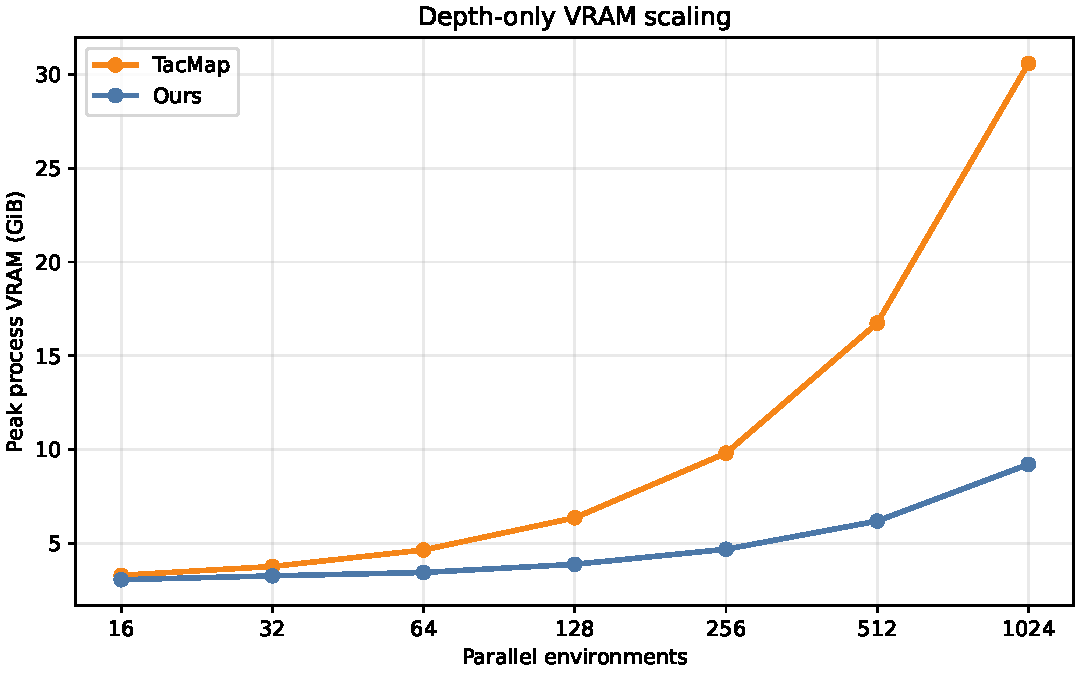
\includegraphics[width=\linewidth]{depth_only_vram_scaling.pdf}
  \caption{Peak process VRAM for depth-only tactile simulation. Ours uses a
  coarse global grid and a contact-driven adaptive window, whereas TacMap uses
  dense rays over the full tactile image.}
  \label{fig:depth_vram_scaling}
\end{figure}

\subsection{Comparison with TacMap-Style Mapping}

TacMap is a geometric depth baseline, not a complete substitute for the
heterogeneous full-hand system.  We therefore compare identical fingertip
regions for depth accuracy and compute, then separately evaluate whether adding
pressure coverage and curved marker motion improves policy performance.

\begin{table*}[t]
\centering
\caption{Comparison with TacMap-style geometric tactile mapping.}
\label{tab:tacmap_method_comparison}
\resizebox{\linewidth}{!}{%
\begin{tabular}{lccccccc}
\hline
Method & Coverage/modalities & Depth RMSE (mm) & Marker EPE (px) & BC success (\%) & RL success (\%) & Real success (\%) & VRAM (GB) \\
\hline
TacMap & Fingertip depth & \TBD{} & -- & \TBD{} & \TBD{} & \TBD{} & \TBD{} \\
TacMap + calibrated real depth & Fingertip depth & \TBD{} & -- & \TBD{} & \TBD{} & \TBD{} & \TBD{} \\
Ours without pressure & Curved depth + marker & \TBD{} & \TBD{} & \TBD{} & \TBD{} & \TBD{} & \TBD{} \\
Ours full & Pressure + curved depth + marker & \TBD{} & \TBD{} & \TBD{} & \TBD{} & \TBD{} & \TBD{} \\
\hline
\end{tabular}%
}
\end{table*}

\subsection{Failure Analysis}

We categorize failures into missed contact, unstable grasp, tangential slip,
depth-domain error, pressure saturation/dead taxels, marker-tracking loss,
latency, and dynamics mismatch.  For each policy, we report the distribution of
failure categories and provide representative synchronized simulation and
hardware traces.  This analysis is necessary to distinguish a perception
failure from a control or dynamics failure.

\section{Limitations}
\label{sec:limitations}

The proposed simulator is a reduced tactile model rather than a general soft
body solver.  It does not reproduce every optical effect, high-frequency
vibration, temperature response, or arbitrary elastomer topology.  Marker
motion depends on calibrated material and friction parameters and may drift
under long contacts.  The current low-resolution geometric map favors policy
throughput over fine texture reconstruction.  Finally, the heterogeneous sensor
layout complicates hardware manufacturing and calibration.  These limitations
are acceptable for the targeted contact-rich control setting, but should not be
interpreted as universal tactile realism.

% ---------------------------------------------------------------------------
% Recommended minimum submission checklist (remove from camera-ready version):
% 1. Do not claim zero-shot transfer until real trials are complete.
% 2. Use >=5 RL seeds and confidence intervals, not a single best curve.
% 3. Add the pressure-only and all-modalities rows; otherwise "full hand" is
%    not supported by the policy ablation.
% 4. Evaluate depth only on registered contact masks, with units in mm.
% 5. Report marker EPE, angle, and temporal drift on paired real trajectories.
% 6. Benchmark without GUI/render-to-disk and state GPU, Isaac version, dt,
%    substeps, environment count, and observation update rate.
% 7. Separate native 32x24 geometry from 320x240 interpolation in all claims.
% 8. Reconcile all descriptive BibTeX keys with verified primary sources.

\begin{thebibliography}{99}

\bibitem{melcer2024feels}
D. Melcer, M. Bombile, and H. M. Clever,
``The F.E.E.L.S.: A dexterous hand with large-area tactile sensing,''
\emph{IEEE Robotics and Automation Letters}, 2024.

\bibitem{yin2023touchdexterity}
Z. Yin, B. Huang, Y. Qin, Q. Chen, and X. Wang,
``Rotating without seeing: Towards in-hand dexterity through touch,''
in \emph{Robotics: Science and Systems}, 2023.

\bibitem{althoefer2024sensorizedskin}
\TBD{Insert the verified Sensorized Soft Skin bibliographic entry.}

\bibitem{wang2022tacto}
S. Wang, M. Lambeta, P.-W. Chou, and R. Calandra,
``TACTO: A fast, flexible, and open-source simulator for high-resolution
vision-based tactile sensors,''
\emph{IEEE Robotics and Automation Letters}, 2022.

\bibitem{si2022taxim}
Z. Si and W. Yuan,
``Taxim: An example-based simulation model for GelSight tactile sensors,''
\emph{IEEE Robotics and Automation Letters}, 2022.

\bibitem{zhao2024fots}
Y. Zhao et al.,
``FOTS: A fast optical tactile simulator for sim-to-real learning of
tactile-guided robot manipulation skills,''
\emph{IEEE Robotics and Automation Letters}, 2024.

\bibitem{akinola2024tacsl}
I. Akinola, J. Xu, J. Carius, D. Fox, and Y. Narang,
``TacSL: A library for visuotactile sensor simulation and learning,''
arXiv:2408.06506, 2024.

\bibitem{su2026tacmap}
L. Su et al.,
``TacMap: Bridging the tactile sim-to-real gap via geometry-consistent
penetration depth map,''
arXiv:2602.21625, 2026.

\bibitem{hydroshear2026}
\TBD{Insert the verified HydroShear author list and venue.}

\bibitem{yin2024tactileskin}
Z. Yin et al.,
``Learning in-hand translation using tactile skin with shear and normal force
sensing,''
arXiv:2407.07885, 2024.

\end{thebibliography}

\end{document}
